\chapter{Evaluation}

TODO describe histogram of number of generated explanations for each existing one, and how this informs design choices

TODO here compare the different approaches, have graphs with results from all algorithms

TODO describe choice of metrics (or do this earlier?)

TODO describe the domains used (or do this earlier?)

TODO discuss hyperthreading and how it affects scaling of performance with number of threads (mention this in background too?)

TODO compare the speedup we get to a perfect $T_1$ to $T_\infty$ speedup

\subsection{XPERIENCE Domain}
TODO

\begin{figure}[!htbp]
\begin{centering}
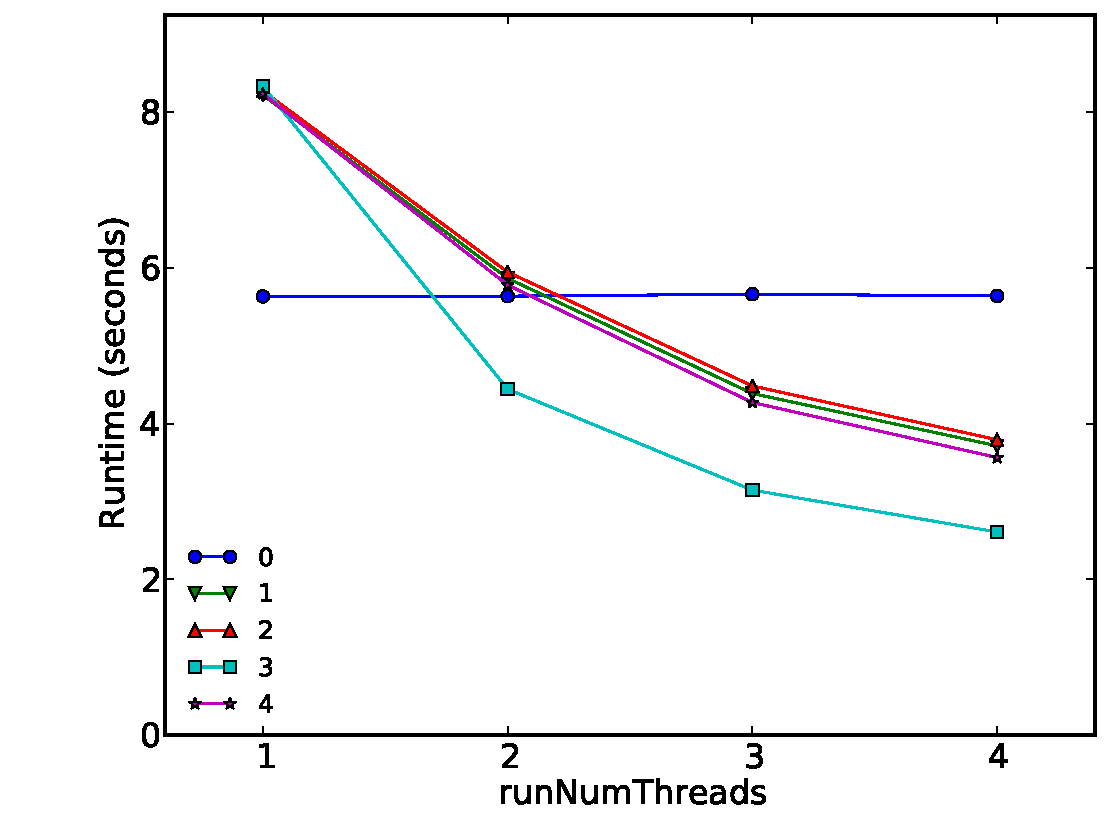
\includegraphics[width=0.8\textwidth]{{{images/threads-xper5-sherlock-all-1}}}
\end{centering}
\caption{Runtime with 1 to 4 threads on Sherlock, All Methods, XPERIENCE domain}
\label{fig:thread-sax-1}
\end{figure}

\begin{figure}[!htbp]
\begin{centering}
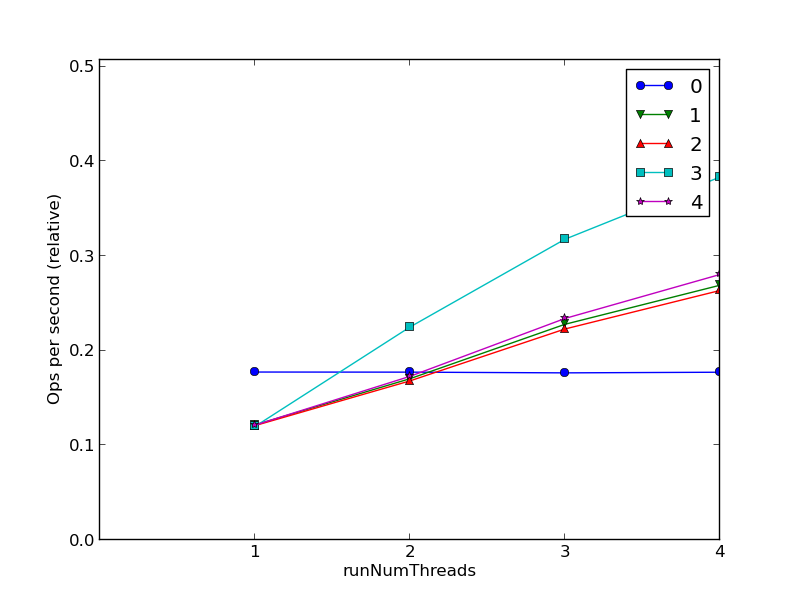
\includegraphics[width=0.8\textwidth]{{{images/threads-xper5-sherlock-all-2}}}
\end{centering}
\caption{Throughput with 1 to 4 threads on Sherlock, All Methods, XPERIENCE domain}
\label{fig:thread-sax-2}
\end{figure}

\begin{figure}[!htbp]
\begin{centering}
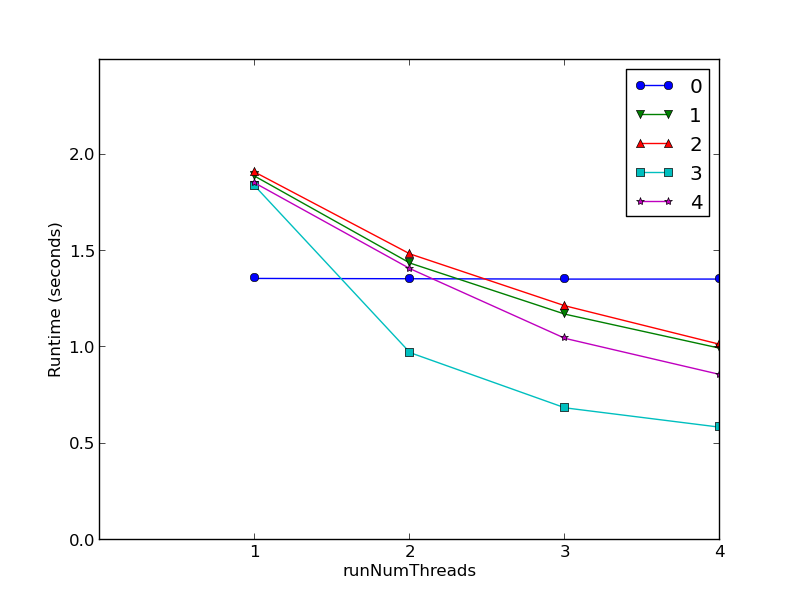
\includegraphics[width=0.8\textwidth]{{{images/threads-log3-sherlock-all-1}}}
\end{centering}
\caption{Runtime with 1 to 4 threads on Sherlock, All Methods, Logistics domain}
\label{fig:thread-sal-1}
\end{figure}

\begin{figure}[!htbp]
\begin{centering}
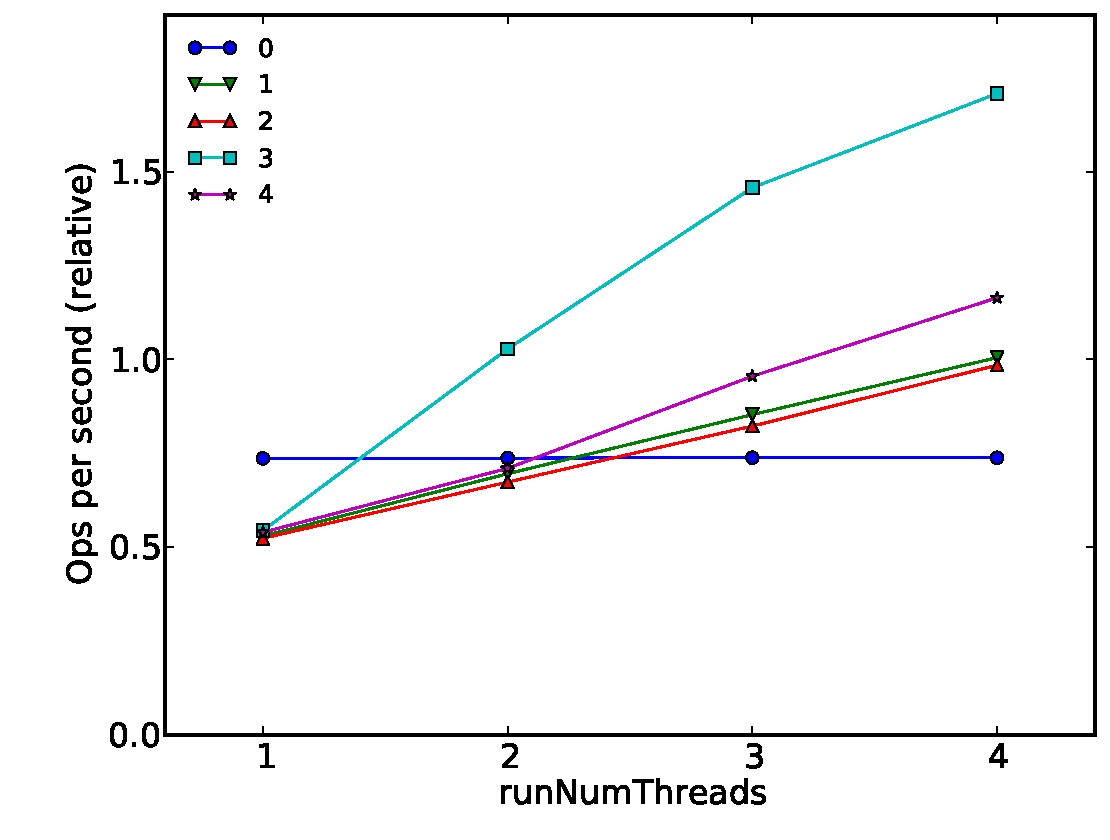
\includegraphics[width=0.8\textwidth]{{{images/threads-log3-sherlock-all-2}}}
\end{centering}
\caption{Throughput with 1 to 4 threads on Sherlock, All Methods, Logistics domain}
\label{fig:thread-sal-2}
\end{figure}

\begin{figure}[!htbp]
\begin{centering}
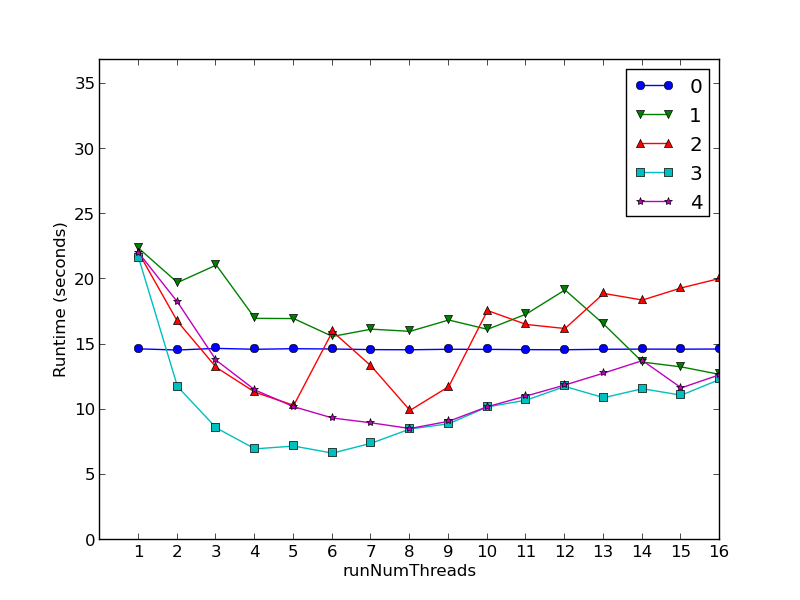
\includegraphics[width=0.8\textwidth]{{{images/threads-xper5-catzilla.inf.ed.ac.uk-all-1}}}
\end{centering}
\caption{Runtime with 1 to 4 threads on Catzilla, All Methods, XPERIENCE domain}
\label{fig:thread-cax-1}
\end{figure}

\begin{figure}[!htbp]
\begin{centering}
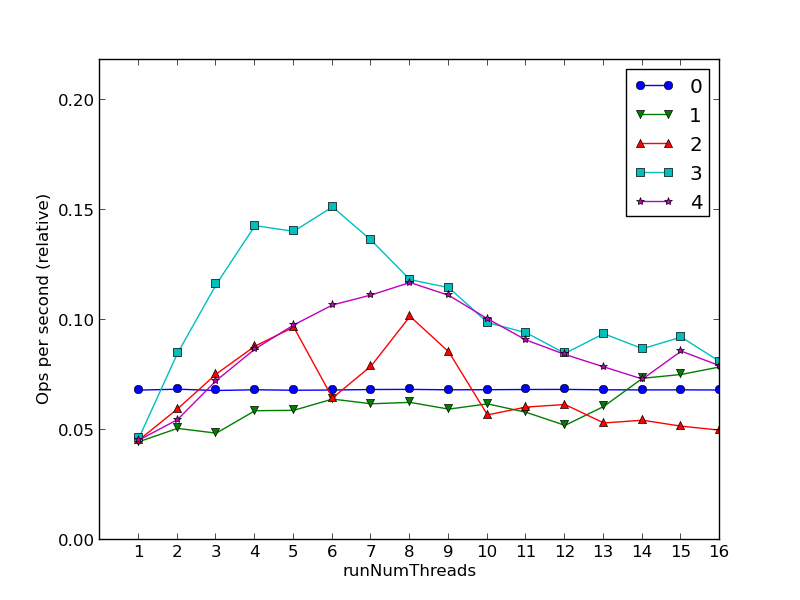
\includegraphics[width=0.8\textwidth]{{{images/threads-xper5-catzilla.inf.ed.ac.uk-all-2}}}
\end{centering}
\caption{Throughput with 1 to 4 threads on Catzilla, All Methods, XPERIENCE domain}
\label{fig:thread-cax-2}
\end{figure}

\begin{figure}[!htbp]
\begin{centering}
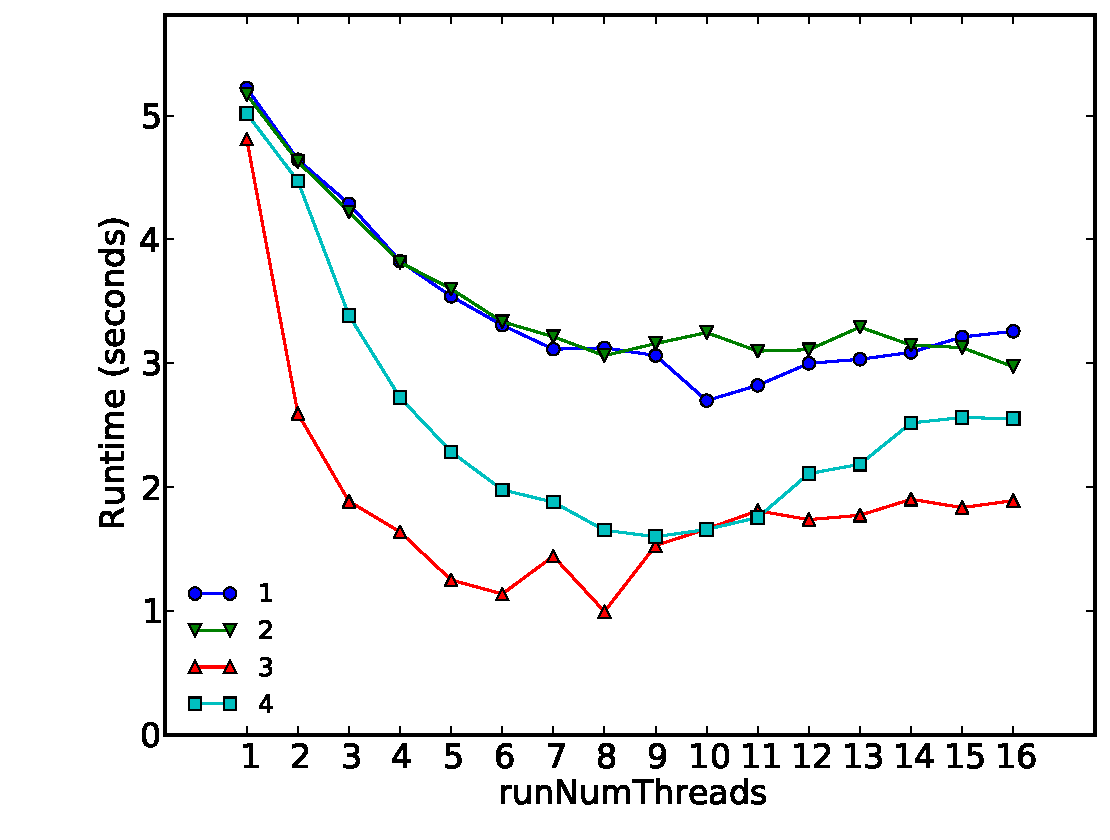
\includegraphics[width=0.8\textwidth]{{{images/threads-log3-catzilla.inf.ed.ac.uk-all-1}}}
\end{centering}
\caption{Runtime with 1 to 4 threads on Catzilla, All Methods, Logistics domain}
\label{fig:thread-cal-1}
\end{figure}

\begin{figure}[!htbp]
\begin{centering}
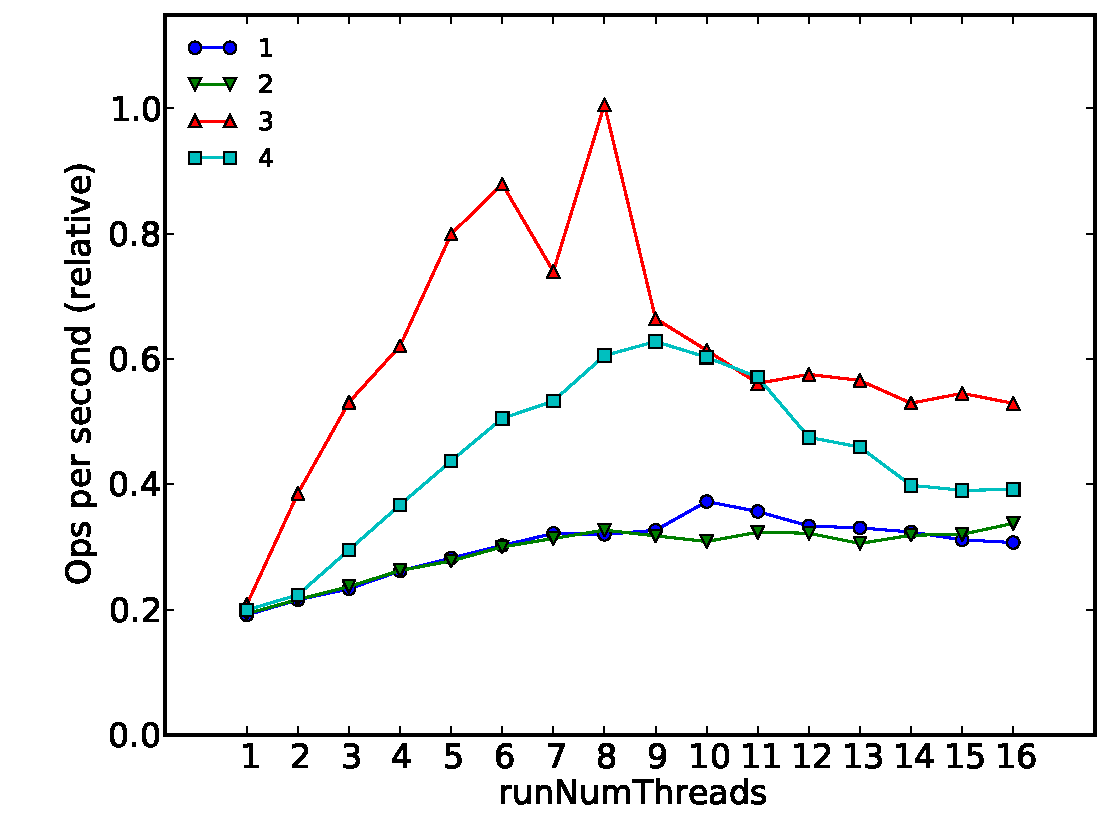
\includegraphics[width=0.8\textwidth]{{{images/threads-log3-catzilla.inf.ed.ac.uk-all-2}}}
\end{centering}
\caption{Throughput with 1 to 4 threads on Catzilla, All Methods, Logistics domain}
\label{fig:thread-cal-2}
\end{figure}